\chapter{ Μεταβλητότητα ακτίνων Χ και ιδιότητες από παρατηρήσεις αρχείου \textlatin{XMM-XXL-North} }
Το πεδίο \textlatin{XMM-XXL} είναι μια περιοχή του ουράνιου θόλου που έχει παρατηρηθεί από το διαστημικό τηλεσκόπιο ακτίνων Χ \textlatin{XMM-Newton} με σκοπό την μελέτη εξωγαλαξιακών πληθυσμών (όπως είναι οι ενεργοί γαλαξιακοί πυρήνες και τα σμήνη γαλαξιών)\cite{2016A&A...592A...1P}. Καλύπτει περίπου $50 $ \textlatin{deg}$^2$ (τετραγωνικές μοίρες) και χωρίζεται σε δύο σχεδόν ίδιου μεγέθους πεδία: το \textlatin{XMM-XXL-North} και το \textlatin{XMM-XXL-South}\cite{2016A&A...592A...1P}. Το πεδίο \textlatin{XMM-XXL} είναι ένα από τα πλέον μεγάλης επιφάνειας εξωγαλαξιακά πεδία ακτίνων Χ, συνεπώς περιέχει έναν σημαντικό αριθμό από λαμπρές πηγές ακτίνων Χ οι οποίες έχουν χαμηλή χωρική πυκνοτητα στο σύμπαν, έτσι, παρατηρήσεις σαν αυτές του \textlatin{XMM-XXL} είναι απαραίτητες για την μελέτη ενός στατιστικά σημαντικού αριθμού ενεργών γαλαξιακών πυρήνων. Οι παρατηρήσεις του \textlatin{XMM-Newton} έχουν γίνει σταδιακά σε χρονικό διάστημα που καλύπτει συνολικά 20 έτη, οπότε έχουμε παρατηρήσεις σε διαφορετικές χρονικές περιόδους που επιτρέπουν την ανάλυση της μεταβλητότητας των \textlatin{AGN} στο πεδίο αυτό.

Το πεδίο \textlatin{XMM-XXL-North} καλύπτει μια περιοχή μεγέθους περίπου $18 $ \textlatin{deg}$^2$ με μέση ορθή αναφορά $02^h 19^m 00^s$ και μέση απόκλιση $ -4^{o}45^{\prime}00^{\prime \prime}$ \cite{2016MNRAS.459.1602L} \cite{2016MNRAS.457..110M}.
Θα μελετήσουμε τις ιδιότητες της μεταβλητότητας στις μαλακές ακτίνες Χ ($0.2-2$ \textlatin{keV}) των πηγών (\textlatin{AGN}) του πεδίου \textlatin{XMM-XXL-North}, μετρώντας την \textlatin{ensemble NXSV} για το πεδίο αυτό και εξετάζοντας πώς η ποσότητα αυτή σχετίζεται με φυσικά μεγέθη του δείγματος. 
%Οι πηγές με  στοχευμένες (\textlatin{pointed}) παρατηρήσεις απεικόνισης του καταλόγου \textlatin{4XMM-DR9}\cite{2020yCat.9059....0W} είναι 11204 στο διάστημα από 3 Φεβρουαρίου 2000 έως 26 Φεβρουαρίου 2019 και εκτείνονται σε ενέργειες $0.2-12\;keV$. 

%{\color{red}AGE: Περισσοτερες πληροφοριες για το ΧΜΜ-ΧΧ: π.χ. το πεδιο ΧΜΜ-ΧΧΛ ειναι μια περιοχη του ουρανου που έχει παρητηρηθει απο τον δορυφορο ακτινων-Χ ΧΜΜ-Νεςτον με σκοπο την μελετη εξωαγαλαξιακν πληθυσμων, π.χ. Ενεργους Γαλαξιακους πυρηνες και σμηνη γαλαξιψν. Βρισκεται σε ουρανιες συντεταγμενες ορθη αναφορα ΧΧΧ και αποκλιση ΧΧΧ και εχει συνολικη επιφανεια ... . Το ΧΜΜ-ΧΧΛ αντιπροσποπευει εαν απο τα πλεον μεγάλης επιφανειας εξωαγαλαγιακα πεδια ακτινών-Χ. Συνεπως περιεχει εαν σημαντικο αριθμο απο λαμπρες πηγεσ ακτινων-Χ, οι οποιές εχουν χαμηλη πυκνότητα (space density) στο Συμπαν και συνεπωρς παρατηρησσεις σαν και αυτες του ΧΜΜ-ΧΧΛ ειναι απαραιτητες για τη μελετη ενος στατιστικα συμαντικου αριθμου. Οι ΧΜΜ παρατηρησεςις που καλυπτουν την επιφανεια του ΧΜΜ-ΧΧΛ έχουν γινει σταδιακα σε περιοδο που καλυπτει συνολικα περιπου 20 χρονια. Συνεπως το πεδιο αυτο εχει παρατηρησεις σε διαφορετικες χρονικες περιοδους που επιτρεπουν την αναλυση της μετβλητοτηας των Ενετργων Γαλαξιακων Πυρηνων στο πεδιο αυτο. }

 \begin{figure}
 \begin{center}
 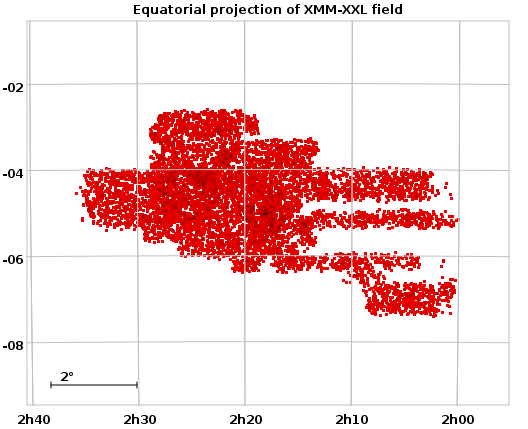
\includegraphics[scale= 0.6]{Figures/EquatorialViewXMMXXL.png}
 \caption{Ισημερινή προβολή του πεδίου \textlatin{XMM-XXL-North}. Ο οριζόντιος άξονας είναι η διορθωμένη για ιδία κίνηση ορθή αναφορά (\textlatin{RA}) και ο κατακόρυφος άξονας η διορθωμένη απόκλιση (\textlatin{Dec}). Προβάλονται οι πηγές με στοχευμένες παρατηρήσεις. (Η εικόνα παράχθηκε χρησιμοποιώντας το πρόγραμμα απεικόνισης \textlatin{TOPCAT} \cite{TopCat} και τον κατάλογο \textlatin{RapidXMM} \cite{RapidXMM}) }
 \label{fig:EquatorialView}
 \end{center}
 \end{figure}

%%%-----------------------------------------------------------%%%%
%%%-----------------------------------------------------------%%%%
%%%-----------------------------------------------------------%%%%

\section{Διαμόρφωση βάσης δεδομένων και διασταύρωση παρατηρήσεων}

%{\color{red}AGE: Επιπλεον χρειαζοτναι πληροφοριες για τον καταλογο ΧΜΜ-ΧΧ που χρησημοποιεις που δεν ειναι απο 4XMM αλλα προερχονται απο την αναλυση των https://ui.adsabs.harvard.edu/abs/2016MNRAS.459.1602L/abstract. Ισως αξιζει να πεις οι υπαρχουν πολλες διαφορετικες ομαδες που εχουν αναλυσει τα δεδομενα του ΧΜΜ στο ΧΜΜ-ΧΧΛ, αλλα εσυ επιλγεςι να χρησημοιποιησεις τον καταλογο απο το παραπανω παπερ. Ο λογος ειναι οτι για αυτο τον καταλογι εχεις στη διαθεση σου επιπλεον πληφοροφια για τις πολυχρωματρικες ιδιοτητες και την ερυθρομετατοπιση των πηγων, https://ui.adsabs.harvard.edu/abs/2017MNRAS.469.3232G/abstract. Επιπλεον θα πρεπει να αναφερθεις στο συνολικο αριθμο πηγων (π.χ. στην 0.5-2keV band, και πόσα απο αυτά εχουν φωτομετρικες και φασματοσκοπικες ερυθρομετατοπισεις.}

Τα δεδομένα του \textlatin{XMM-Newton} στο πεδίο \textlatin{XMM-XXL-North} έχουν αναλυθεί από πολλές ερευνητικές ομάδες. Εμείς επιλέγουμε να εργαστούμε με τον κατάλογο που συνοδεύει η εργασία \textlatin{<<X-ray spectral properties of the AGN sample in the northern XMM-XXL field>> (Liu et al. 2016)}\cite{2016MNRAS.459.1602L}, ο λόγος είναι ότι για τον κατάλογο αυτό έχουμε στην διάθεσή μας πληροφορία για τις πολυχρωματικές ιδιότητες και την ερυθρομετατόπιση των πηγών όπως συμπληρώνει η εργασία  \textlatin{<<X-ray constraints on the fraction of obscured active galactic nuclei at high accretion luminosities>> (Georgakakis et al. 2017)}\cite{2017MNRAS.469.3232G}.
Ο αρχικός κατάλογος αυτός έχει παρατηρήσεις από 8445 στοχευμένες πηγές. Από αυτές τις πηγές για τις 3129 έχουμε φασματοσκοπική μέτρηση ερυθρομετατόπισης, ενώ για άλλες 1854 έχουμε φωτομετρική μέτρηση ερυθρομετατόπισης (χωρίς να έχουμε φασματοσκοπική για τις τελευταίες). Έτσι από τις 8445 πηγές του αρχικού καταλόγου για τις 4983 έχουμε πληροφορία ερυθρομετατόπισης, ενώ για 3462 από αυτές δεν έχουμε καθόλου πληροφορία ερυθρομετατόπισης.

\subsection{Βάση δεδομένων \textlatin{RapidXMM}}

Για την μελέτη της μεταβλητότητας απαιτείται ένας κατάλογος που περιέχει πληροφορίες για την ένταση κάθε πηγής σε ξεχωριστές παρατηρήσεις και που περιλαμβάνει φωτομετρικές πληροφορίες για όλες τις παρατηρήσεις του \textlatin{XMM-Newton}. 
Θα χρησιμοποιήσουμε τον κατάλογο \textlatin{RapidXMM database} που συνοδεύει την εργασία \textlatin{<<The RapidXMM Upper Limit Server: X-ray aperture photometry of XMM-Newton archival observations>> (Ruiz et al. 2021)} \cite{RapidXMM}, ο κατάλογος αυτός αναπτύχθηκε για να παρέχει άνω όρια ροής για το τμήμα του ουρανού που καλύπτεται από τον \textlatin{XMM-Newton}, όμως περιλαμβάνει επιπλέον ποσότητες οι οποίες μπορούν να χρησιμοποιηθούν για τον υπολογισμό ροής (φωτομετρία) ων παρατηρούμενων πηγών. Ο κατάλογος αυτός περιέχει 63162 παρατηρήσεις από 8436 καταγεγραμμένες πηγές, σε μαλακές ($0.2-2$ \textlatin{keV}) και σκληρές ($2-12$ \textlatin{keV}) ακτίνες Χ, από τρία διαφορετικά όργανα: \textlatin{PN, MOS1, MOS2}.  
Θα επικεντρωθούμε σε στοχευμένες παρατηρήσεις του πεδίου \textlatin{XMM-XXL-North} και συγκεκριμένα σε ακτινοβολία που έχει καταγραφεί στο ενεργειακό παράθυρο $0.2-2$ \textlatin{keV}, δηλαδή ακτινοβολία μαλακών ακτίνων Χ.

Το \textlatin{RapidXMM} χρησιμοποιεί το σύστημα \textlatin{pixelisation HEALPix}, το σύστημα αυτό διαιρεί την γεωμετρική προβολή της σφαίρας σε ισεμβαδικά \textlatin{pixel} και προσφέρει μια ένα-προς-ένα απεικόνιση μιας δι-διάστατης κατανομής στοιχείων διακριτού εμβαδού σε μία μονοδιάστατη συστοιχία ακεραίων αριθμών. Η συστοιχία ακεραίων επιδέχεται δύο διαφορετικούς τρόπους αρίθμησης \textlatin{RING} και \textlatin{NESTED} καθώς και διαφορετική ευκρίνεια (μέγεθος \textlatin{pixel}). Έτσι στον θόλο προβάλεται ένα νοητό πυκνό πλέγμα που σχηματίζει <<κελιά>>. Επιλέγεται ο τρόπος αρίθμησης \textlatin{NESTED} και η παράμετρος ευκρίνειας $16$ η οποία αντιστοιχεί σε μέγεθος κελιού $3.2$ \textlatin{arcsec}, που είναι συγκρίσιμο με την ευκρίνεια των εικόνων του συστήματος \textlatin{Pipeline Processing Subsystem (PPS)} του \textlatin{XMM-Newton} οι οποίες έχουν μέγεθος \textlatin{pixel} $4.44$ \textlatin{arcsec}.\\
Για κάθε μία από αυτές τις θέσεις δίνονται μεταξύ άλλων: καταμέτρηση φωτονίων πηγής στο διάφραγμα για κάθε ενεργειακή μπάντα, καταμέτρηση φωτονίων υποβάθρου για κάθε ενεργειακή μπάντα, χρόνος έκθεσης παρατήρησης για κάθε ενεργειακή μπάντα, ανιχνευτής με τον οποίο έγινε η παρατήρηση, κλάσμα της κατανομής ροής σημειακής πηγής που περιέχεται στο διάφραγμα, ημερομηνία και ώρα έναρξης και λήξης της παρατήρησης, ο λόγος εμβαδών διαφράγματος παρατήρησης πηγής προς διάφραγμα μέτρησης υποβάθρου.

%{\color{red}AGE: ο \textlatin{RapidXMM} ειναι για τη φωτομετρια. Η αναλυση των παρατηρησεων από τοτς Liu et al., δεν περιλεμβανει πληροφορια για την μεταβλητοτα των πηγων. Οι Liu et al. συνενωσαν ολες τιςε παρατηρησεις με αλλιλοεπικαλυψη με σκοπο την αυξηση του συνολικου χρονου εκθεσης και την ανιχνευση αμυδρων πηγων. Ο καταλογος που δινει την μεση ροη καθε πηγης οπως προκυπτει απο την συννενσωη ολων των παρατηησων σε διαφορετικες εποχες (χρονικες στιγμες). Για τη μελετη της μεταβλιτοτηας απαιιητετα ενας καταλογος ο οποιος θα περιχει πληροφοριες για την ενταση καθε πηγης σε ξεχωριστες εποχες παρατηρησεις. Για το λογο αυτο χρησημοποιουμε εναν νεο καταλογο που παριλαμβανει  φωτομεττιες πληρογοριες για ολες τις ξεχωριστες παρατηρησεισ του ΧΜΜ...  Ο βασικος στοχος της αναπτηξης του \textlatin{RapidXMM} ειναι η διμιοθργια μιας βαση δεδομεμνω που θα περιεχει ανω ορια ροης σε ολο το τμημα του ουρανου που καλυπτεται απο τον ΧΜΜ. Η βαση αυτη ομως περλιμαβνει επιπλεον ποσοτητς οι οποιες μπορουν να χρησημοποιηθουν για τον υπολογιμσο της ροης πηγων (φωτομετρια). Αυτη περιλαμβανει extracted counts within an aperture of 30", the expected background level within the same aperture, the corresping expsore time...} 

%{\color{red}AGE: το \textlatin{RapidXMM} χρησημοποει το \textlatin{pixelisation HEALPix} οποτε ισως καλυτερα να το πριγραψεις εδω σε σχεση με το \textlatin{RapidXMM}. Επιπλεον πρεπει να πεις οτι η ευκερινια του  \textlatin{RapidXMM}  ειναι περιπου 3.2" που αβτιστοχει σε παράμετρο ευκρίνειας $16$. Μπορεις να πεις το \textlatin{RapidXMM} παρεχει τις παραπανω φωτομετρικες πληρογοριες σε ενα πυκνο πλεγμα (grid) απο θεσεις που αντιστοιχουν σε 3.4". Σε καθε μια απο αυτεσ τις θεσεις δινονατι οι εξεις πληροφοριες, aperture coutnts ,.... }

%%%-----------------------------------------------------------%%%%
\subsection{Αντιστοίχιση πηγών και πληροφορίες από άλλους καταλόγους}

Όπως τονίσαμε, ενώ βασιζόμαστε στις ποσότητες του καταλόγου \textlatin{RapidXMM}, χρησιμοποιούμε πληροφορίες ροής και ερυθρομετατόπισης από τον κατάλογο που συνοδεύει την εργασία \textlatin{<<X-ray constraints on the fraction of obscured active galactic nuclei at high accretion luminosities>> (Georgakakis et al. 2017)}.\\
Για να διασταυρώσουμε τις πληροφορίες αυτές με τις πηγές του \textlatin{RapidXMM}, εισάγουμε τις ουρανογραφικές (\textlatin{ICRS}) συντεταγμένες (\textlatin{RA}, \textlatin{Dec}) και μέσω του συστήματος \textlatin{HEALPix} με αρίθμηση \textlatin{pixel NESTED} και παράμετρο ευκρίνειας $16$ αντιστοιχίζουμε κάθε παρατήρηση σε έναν αριθμό ταυτοποίησης \textlatin{HEALPix}.\\
Βάσει του αριθμού αυτού, ο οποίος σηματοδοτεί μια πηγή (\textlatin{AGN}), διασταυρώνουμε παρατηρήσεις του καταλόγου \textlatin{RapidXMM database} με τις μετρήσεις ροής ενέργειας (\textlatin{flux}) και ερυθρομετατόπισης (\textlatin{redshift}). Αποτέλεσμα είναι να εμπλουτίσουμε τον κατάλογο \textlatin{RapidXMM database} με πληροφορίες για \textlatin{redshift} και \textlatin{flux} (όπου \textlatin{flux} είναι η μέση ροή κάθε πηγής που προκύπτει από όλες τις χρονικές παρατηρήσεις του \textlatin{XMM-Newton} που αντιστοιχούν σε αυτήν), όπου αυτά υπάρχουν, και να απορρίψουμε παρατηρήσεις του καταλόγου αυτού για τις οποίες δεν έχουμε τις πληροφορίες αυτές.\\
Στην εργασία αυτή θα επικεντρωθούμε σε παρατηρήσεις του ανιχνευτή ΡΝ σε μαλακές ακτίνες Χ (δηλαδή στο ενεργειακό παράθυρο $0.2-2$ \textlatin{keV}).
Ο κατάλογος \textlatin{RapidXMM} περιέχει 8436 πηγές (από τις 8445 του αρχικού καταλόγου) από τις οποίες οι 8299 έχουν παρατηρήσεις από τον ανιχνευτή ΡΝ. Από τις 8299 πηγές αυτές οι 3092 έχουν μέτρηση φασματοσκοπικής ερυθρομετατόπισης, ενώ άλλες 1830 έχουν φωτομετρική μέτρηση ερυθρομετατόπισης. Δηλαδή από τις 8299 πηγές με παρατηρήσεις στον ανιχνευτή ΡΝ του καταλόγου \textlatin{RapidXMM database} για τις 4922 έχουμε πληροφορία ερυθρομετατόπισης, ενώ για τις 3377 δεν έχουμε πληροφορία ερυθρομετατοπισης.

%{\color{red}AGE: οι πηγες προεχρονται απο τον καταλογο των \textlatin{Liu et al. 2016} και οχι απο το  \textlatin{4XMM-DR9}. Επιπλεον η φωτομετρια δεν τατθοποιεις τις πηγες με τη ροη απο το 4ΧΜΜ αλλα αντιθετα υπολογιζεις τη φωτομετρια απο το ραπιδ. Εδω περιγραφεις πως κανεις query με ra, dec ωστε να βρεις τα αντιστοιχα \textlatin{HEALPix} πιξελ πανω στα οποια βρισκονταο οι πηγες. Εαν μια πηγη εχει παρτηρηθεο σε περισσιτερες απο μια ξεχωριστες ΧΜΜ-Νεςτον παρατηρησεις η βαση δεδοεμενων  \textlatin{RapidXMM}  επιστρεφει για καθε μια απο τις αυτες: (α) συνολικο αριθμο από φωτονια σε καθε μια απο τις πανρες .... (β) .... (γ)....  Οι τιμες αυτες ειναι δυνατο να συνδιαστουν για τον υπολογισμο της παρατηρουμενης ροης της πηγης σε ξαθε ξεωχιστη παρατηρση. Επισης μπορεις να πεις εδω οτι χρησημοποιεις μονο PN kai 0.2-2keV.}

%%%-----------------------------------------------------------%%%%
%%%-----------------------------------------------------------%%%%
%%%-----------------------------------------------------------%%%%
\section{Υπολογισμός ποσοτήτων}

%{\color{red}AGE: Ισως θα μπορουσες να ξεινησεις απο την φωτομετρια της CR=(N-B)/t/EEF, Εξηγεις τη ειναι η καθε μια ποσοτητα. Στηη συνεχεια εξηγεις πως υπολογιζεται το Β, και μονο τοτε αναφρεις την προσσεγιση dB=sqrt(B) και εξηγεις οτι η κατανομη ειναι Poisson. Επισης στη συνεχεια και την αβεβαιοτητα. Επισης πρεπει να πεις οτι το CR εχει μοναδες photo/s kai oxi erg/s/cm2 (energy flux) και συνεπως δεν περιλμαβνει υποθεσεις για το φασμα της πηγης.}

\subsection{\textlatin{Count rate} και αβεβαιότητα}

Για την φωτομετρία στις ακτίνες Χ, ως ροή δεν χρησιμοποιούμε το μέγεθος της ενεργειακής ροής (\textlatin{flux}) που μετράται σε \textlatin{erg s}$^{-1}$ \textlatin{cm}$^{-2}$, αλλά χρησιμοποιούμε το μέγεθος του ρυθμού καταγραφής φωτονίων (\textlatin{count rate}) που μετρά φωτόνια (κυματοπακέτα) ανά μονάδα χρόνου \textlatin{photon counts} $\cdot$ \textlatin{s}$^{-1})$. Το μέγεθος αυτό είναι καθαρά φωτομετρικό και δεν περιλαμβάνει καμία παραδοχή για το φάσμα της πηγής.\\
Όπως είδαμε και στην ενότητα 3.7.3, οι παρατηρήσεις των πηγών που μελετάμε έγιναν με άνοιγμα διάφραγματος ακτίνας $15$ \textlatin{arcsec} ενώ για την καταγραφή του υποβάθρου το άνοιγμα του διαφράγματος είναι δακτύλιος μεταξύ ακτίνων $60$ και $180$ \textlatin{arcsec}.

To \textlatin{Count Rate} για κάθε παρατήρησή μας δεδομένης ενεργειακής μπάντας (εδώ $0.2-2$ \textlatin{keV}) και για δεδομένο όργανο παρατήρησης (εδώ \textlatin{EPIC PN})\cite{RapidXMM}:
\begin{equation} CR = \frac {(T-B)} { t_{exp}  \cdot EEF}  \label{eq:CR} \end{equation}

Όπου:\\
$T$ : η συνολική καταμέτρηση φωτονίων (\textlatin{total realised counts}) στο διάφραγμα ($15$ \textlatin{arcsec} για στοχευμένες παρατηρήσεις)\\ 
$B$ : υπόβαθρο (\textlatin{background})\\
$t_{exp}$ : χρονικό διάστημα διάρκειας μεμονομένης παρατήρησης \\
$\mbox{EEF}$ : κλάσμα ενέργειας της \textlatin{PSF} της παρατήρησης που περικλείεται στο διάφραγμα ακτίνας $15$ \textlatin{arcsec}

Η αβεβαιότητα στον υπολογισμό $CR$ για κάθε παρατήρηση εκτιμάται σύμφωνα με την διάδοση σφαλμάτων\cite{BuchnerGeorgakakis} (αν θεωρήσουμε το $CR$ ως συνάρτηση των μεταβλητών $Τ$ και $Β$, $CR(T,B) = \frac {(T-B)} { t_{exp}  \cdot EEF} $):     
  \begin{equation} CR_{err} = \sqrt{ \Big( \frac{\partial CR}{\partial T} \Big)^2 \cdot T_{err}^2  +  \Big( \frac{\partial CR}{\partial B} \Big)^2 \cdot B_{err}^2   } = \frac{1}{t_{exp} \cdot EEF} \sqrt{  T_{err}^2 + B_{err}^2    } \label{eq:CRerr} \end{equation}
  
Όπου:\\
$T_{err} = \delta T$ : η αβεβαιότητα στην συνολική καταμέτρηση φωτονίων (\textlatin{total realised counts}) στο διάφραγμα ($15$ \textlatin{arcsec} για στοχευμένες παρατηρήσεις)\\ 
$B_{err} = \delta B$ :  η αβεβαιότητα στo \textlatin{background} (θα συζητηθεί παρακάτω)

Για να υπολογίσουμε την στατιστική αβεβαιότητα στα \textlatin{total realised counts} θα χρησιμοποιήσουμε την προσέγγιση \textlatin{Gehrels}\cite{1986ApJ...303..336G}.
\begin{equation} \delta T \approx 1+\sqrt{T+0.75 } \label{eq:Gehrels} \end{equation}
Η προσέγγιση αυτή είναι χρήσιμη για υπολογισμό άνω ορίων διαστήματος αξιοπιστίας σε περιπτώσεις μικρού πλήθους γεγονότων (π.χ. μικρό πλήθος καταγεγραμμένων φωτονίων) στατιστικού δείγματος.

Η παραπάνω έκφραση για τον ρυθμό καταγραφής φωτονίων (εξίσωση \ref{eq:CR}) προκύπτει επειδή (αν $S$ to σήμα της πηγής) η συνεισφορά του σήματος της πηγής στο πλήθος παρατηρούμενων φωτονίων στο διάφραγμα εξαρτάται από το σχήμα της \textlatin{PSF} και από τον χρόνο παρατήρησης. Αν το εγγενές \textlatin{Count Rate} μιας πηγής είναι $CR$, τότε το σήμα πηγής $S$\cite{RapidXMM}:
\begin{equation}
    S = CR \cdot t_{exp}  \cdot EEF \label{eq:sourcesignal}
\end{equation}
Ο καταγραφόμενος αριθμός φωτονίων $T$ στο διάφραγμα είναι υλοποίηση μιας διαδικασίας \textlatin{Poisson}, με αναμενόμενη τιμή $\lambda = S + B$.   

%%%-----------------------------------------------------------%%%%

\subsection{Ακτινοβολία υποβάθρου και αβεβαιότητα}

Η καταγραφή και καταμέτρηση φωτονίων (γεγονότων) και ο υπολογισμός του ρυθμού πραγματοποίησης των γεγονότων αυτών διέπονται από στατιστική \textlatin{Poisson}. Όταν έχουμε σχετικά υψηλό αριθμό γεγονότων, τότε έχουμε αντιστοίχηση με στατιστική \textlatin{Gauss} (για περισσότερα γεγονότα έχουμε αντιστοίχιση σε περισσότερα $\sigma$)\cite{1986ApJ...303..336G}. Για να εκτιμήσουμε το υπόβαθρο, καταγράφουμε φωτόνια σε μεγαλύτερο διάφραγμα και έπειτα τα συρρικνώνουμε με τον λόγο των εμβαδών των διαφραγμάτων. Στην βάση δεδομένων μας, διαθέτουμε το κλάσμα φωτονίων υποβάθρου που αντιστοιχεί στην παρατήρηση και τον λόγο εμβαδών, έτσι συμπεραίνουμε το υπόβαθρο στην συλλογή μεγάλου διαφράγματος (χρησιμοποιώντας όλην την πληροφορία που συλλέχθηκε) και υπολογίζουμε την αβεβαιότητα με καλή προσέγγιση στατιστικής \textlatin{Gauss}, έπειτα χρησιμοποιώντας τον λόγο των εμβαδών εκτιμούμε την αβεβαιότητα στην κλίμακα της παρατήρησης.
Το ανηγμένο υπόβαθρο $B_{poisson}$:
\begin{equation}
    B_{Rapid} = B_{poisson}  \cdot \frac {A_{source} }{A_{backgr}} \iff B_{poisson} =   \dfrac{ B_{Rapid} }{\frac {Α_{source} }{Α_{backgr}} } \label{eq:Background}
\end{equation}
H αβεβαιότητα ανηγμένου υποβάθρου στην προσέγγιση \textlatin{Gauss} $\delta B_{poisson}$:
\begin{equation}
     \delta B_{poisson} = \sqrt{ B_{poisson}} =\sqrt{ \dfrac{ B_{Rapid} }{\frac {Α_{source}}{Α_{backgr}} }}
\end{equation}
H αβεβαιότητα στο διάφραγμα της παρατήρησης, από την αβεβαιότητα ανηγμένου υποβάθρου:
\begin{equation}
     \delta B_{Rapid} = \delta B_{poisson} \cdot \frac {A_{source} }{A_{backgr}}= \sqrt{ \dfrac{ B_{Rapid} }{\frac {Α_{source}}{Α_{backgr}} }}\cdot \frac {A_{source} }{A_{backgr}} \label{eq:Berr}
\end{equation}
%%%-----------------------------------------------------------%%%%

\subsection{\textlatin{Signal-to-Noise ratio} }
Για κάθε μια παρατήρηση ο λόγος σήματος προς θόρυβο \textlatin{Signal-to-Noise ratio (S/N)}:   
\begin{equation}   S/N = \frac{T-B}{\sqrt{\delta T^2 + \delta B^2}} \end{equation}
Όπου:\\     
$T$ :  η συνολική καταμέτρηση φωτονίων (\textlatin{total realised counts}) στο διάφραγμα \\
$B$ : \textlatin{background}  \\   
$\delta T$ : η αβεβαιότητα στα \textlatin{total realised counts} (Βλ. εξίσωση \ref{eq:Gehrels})\\
$\delta B$ : η αβεβαιότητα στο \textlatin{background} (Βλ. εξίσωση \ref{eq:Berr})

Έτσι για κάθε μία παρατήρηση κάθε πηγής μπορούμε να έχουμε και μια τιμή \textlatin{S/N}.
Ενώ μπορούμε σε κάθε μία πηγή (\textlatin{HEALPix ID}) να αναθέσουμε μία συσσωρευμένη τιμή \textlatin{S/N} συγκεντρώνοντας τις μετρήσεις όλων των παρατηρήσεων που αντιστοιχούν σε κάθε πηγή ως εξής:
 \begin{equation} {S/N}_{stacked} =   \dfrac { \sum_1^N T_i -  \sum_1^N  B_i}{\sqrt{ \big(\sum_1^N \delta T_i \big)^2 + \big(\sum_1^N \delta B_i \big)^2}} \label{eq:SNstacked}\end{equation} 
 
Στο εξής όταν αναφερόμαστε σε τιμή \textlatin{S/N} μίας πηγής, θα αναφερόμαστε στον υπολογισμό της εξίσωσης \ref{eq:SNstacked}.
   
%%%-----------------------------------------------------------%%%%
\subsection{\textlatin{Νormalised Excess Variance} και αβεβαιότητα }

H \textlatin{excess variance (NXSV)} μετρά πόση από την ολική ροή είναι μεταβλητή, αφού αφαιρέσουμε το στατιστικό σφάλμα. Το \textlatin{Count Rate (CR)} είναι υποτυπώδης ροή ως ρυθμός καταμέτρησης φωτονίων. Χρησιμοποιώντας τον παρακάτω τύπο, υπολογίζουμε για κάθε πηγή- δηλαδή για κάθε ξεχωριστό αριθμό \textlatin{HEALPix}- την ποσότητα \textlatin{NXSV} για παρατηρήσεις στην ενεργειακή μπάντα $0.2-2$ \textlatin{keV} \cite{1997ApJ...476...70N}: 
    \begin{equation} \sigma^2_{rms} = \frac{1}{N \cdot {\bar x}^2 }   \sum_{i=1}^{N}  [ (x_i -\bar x)^2  - x_{err, i}^2]  \label{eq:NXSV}\end{equation}
Όπου:\\
$N$ : πλήθος παρατηρήσεων που αντιστοιχούν σε μία πηγή \\                              
$x_i$ : \textlatin{Count Rate} μιας μεμονομένης παρατήρησης \\             
$\bar x$ : αριθμητικός μέσος όρος \textlatin{Count Rate} από παρατηρήσεις που αντιστοιχούν σε μία πηγή\\ 
$x_{err, i}$ : στατιστικη αβεβαιότητα στο \textlatin{Count Rate} μιας μεμονομένης παρατήρησης (όπως την υπολογίσαμε σε παραπάνω ενότητα, εξίσωση \ref{eq:CRerr} )  %{\color{red}(δωσε τον αριθμο του equation) λογω του σφαλμαοτς μετησεις}\\

Η αβεβαιότητα στην \textlatin{NXSV} ($\sigma^2_{rms}$) είναι $  \sigma^2_{rms, err}$, αναπαριστά τα σφάλματα μέτρησης σε εκτιμήσεις της \textlatin{NXSV} από προσομοιώσεις καμπύλων φωτός και υπολογίζεται από την εξής εμπειρική σχέση\cite{2003MNRAS.345.1271V}:     
  
\begin{equation}  \sigma^2_{rms, err} = \sqrt{ \Big( \sqrt{\frac{2}{N}}\cdot \frac{\overline{ x^2_{err} }}{\bar{x}^2} \Big)^2 + \Big( \sqrt{ \frac{\overline{ x^2_{err}}}{N}    }   \cdot \frac{2F_{var}}{\bar x}  \Big)^2  }  \label{eq:NXSVerr} \end{equation}

$N$ : πλήθος παρατηρήσεων που αντιστοιχούν σε μία πηγή \\
Όπου η ποσότητα $\overline{ x^2_{err}}$ είναι η μέση τετραγωνική αβεβαιότητα στο \textlatin{Count Rate}:     
\begin{equation}  \overline{ x^2_{err}} =   \frac{1}{N }   \sum_{i=1}^{N} x_{err, i}^2  \end{equation}
 
Και η ποσότητα $F_{var} $ είναι το κλασματικό πλάτος της \textlatin{NXSV}:    
\begin{equation} F_{var} = \sqrt{ \frac{ \sigma^2_{rms} -  \overline{ x^2_{err}}   } {{\bar x}^2}  }     \end{equation}
Έτσι, η κάθε μέτρηση \textlatin{NXSV} για κάθε πηγή συνοδεύεται με τον αντίστοιχο υπολογισμό για την αβεβαιότητα της \textlatin{NXSV}.

  \begin{figure*}
 \begin{center}
 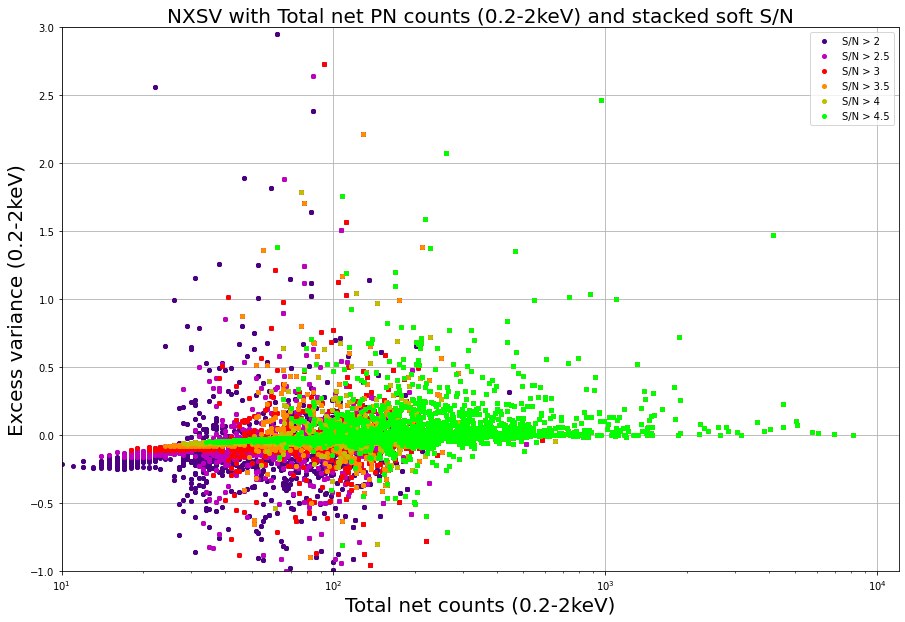
\includegraphics[width=0.9\linewidth]{Figures/NXSV_Counts_zweight.png}
 \caption{\textlatin{NXSV} με συνολικές καταμετρήσεις φωτονίων στο διάφραγμα κατά \textlatin{redshift.}}
 \label{fig:NXSV_counts}
 \end{center}
 \end{figure*}

Όπως βλέπουμε στην εξίσωση \ref{fig:NXSV_counts}, στούς υπολογισμούς μας έχουμε τιμές της \textlatin{NXSV} οι οποίες είναι αρνητικές, αυτό συμβαίνει διότι όπως φαίνεται στον τύπο \ref{eq:NXSV}, η τετραγωνική αβεβαιότητα μεμονομένων παρατηρήσεων \textlatin{CR} είναι μεγαλύτερη από το τετράγωνο της απόστασής τους από την μέση τιμή των παρατηρήσεων της πηγής στην οποία αντιστοιχούν. Όπως βλέπουμε στο σχήμα \ref{fig:NXSV_counts} αυτό αντιμετωπίζεται σε μεγάλο βαθμό αν απορρίψουμε πηγές με μικρό \textlatin{S/N}, καθώς ο θόρυβος σήματος συνεισφέρει σημαντικά στην αβεβαιότητα της μέτρησης. 

%%%-----------------------------------------------------------%%%%
\subsection{Λαμπρότητα και \textlatin{redshift}}

Έχοντας πληροφορίες για ερυθρομετατόπιση και ροή στην ενεργειακή μπάντα $0.2-2$ \textlatin{keV} \cite{2017MNRAS.469.3232G}, υπολογίζουμε απόσταση και λαμπρότητα για κάθε μία πηγή (\textlatin{AGN})\cite{2006PASP..118.1711W}. Χρησιμοποιούμε τις κοσμολογικές παραμέτρους $H_0 = 70$ \textlatin{km  s}$^{-1}$ \textlatin{Mpc}$^{-1}$, $\Omega_m = 0.3$ , $\Omega_v=0.7$ και επίπεδο Σύμπαν.\\
Για δεδομένο \textlatin{redshift}, $z$, ο παράγοντας κλίμακας του Σύμπαντος:   $a = \dfrac{1}{1+z}$\\
Η αδρανειακή ακτινική απόσταση (\textlatin{comoving radial distance}- απόσταση που μετράμε στο αδρανειακό μας σύστημα ως παρατηρητές)\cite{2006PASP..118.1711W}:
\begin{equation}
D_{cmr} =  \int \frac{c dt}{a} = \int_{1/(1+z)}^1 \frac {cda}{a\dot a}
\end{equation}

Η απόσταση που διανύει το φώς (\textlatin{light travel time distance}- χρόνος φωτός από την εκπομπή του μέχρι την καταγραφή του σήματος)\cite{2006PASP..118.1711W}:
\begin{equation} D_{ltt} =  \int c dt = \int_{1/(1+z)}^1 \frac {cda}{\dot a} \end{equation}

Θεωρούμε ποσότητα $X$ τέτοια ώστε: \begin{equation} \dot a = H_o \sqrt X \end{equation}
Για επίπεδο Σύμπαν ($\Omega_{tot}=1$), με $\Omega_m$, $\Omega_v$ (ύλη και κενό μόνο) η ποσότητα αυτή γίνεται:    
\begin{equation} X(a) = \frac{\Omega_m}{a} + \frac{\Omega_r}{a^2} + \Omega_{v} a^2 + (1-\Omega_{tot}) \iff X(a) = \frac{\Omega_m}{a} + \Omega_v a^2 \end{equation}  

Έτσι, η αδρανειακή ακτινική απόσταση:
\begin{equation} 
\begin{aligned}
D_{cmr} =  {} &  \int_{1/(1+z)}^1 \frac {c }{a\cdot H_o \sqrt X} da = \frac{c}{H_o}  \int_{z}^0  (1+z) \cdot \frac{1}{\sqrt{\Omega_m/a + \Omega_v a^2 }} d \big( \frac{1}{1+z} \big) = \\
& =\frac{c}{H_o}  \int_{z}^0  \frac{(1+z)}{\sqrt{\Omega_m/a + \Omega_v a^2 }} \Big( \frac{-1}{(1+z)^2} \Big) dz = % \end{equation}
%\begin{equation} =  
\frac{c}{H_o}  \int_0^{z} \frac{1}{(z+1) \sqrt{\Omega_m/a + \Omega_v a^2 }} dz = \\ & =\frac{c}{H_o}  \int_0^{z} \frac{1}{(z+1) \sqrt{\Omega_m (1+z) + \Omega_v / (1+z)^2 }} dz \label{eq:Dcmr}
\end{aligned}
\end{equation}

Η απόσταση γωνιακής διαμέτρου $ D_{A} = \frac{R}{\theta}$ (\textlatin{angular size distance}- το εγκάρσιο ιδιομήκος $R$ ένος αντικειμένου που υποτείνει γωνία $\theta$):
 $D_{A} =  \frac{D_{cmr}}{(1+z)}  $

Η απόσταση λαμπρότητας (\textlatin{luminosity distance}- ορίζεται ώστε ο νόμος αντιστρόφου τετραγώνου για βολομετρικές ροές $F_{bol} = L/(4\pi D_L^2)$ να λειτουργεί πλήρως)\cite{2006PASP..118.1711W}: 
\begin{equation}  D_L = (1+z)^2 D_A = (1+z) D_{cmr} \label{eq:DL}\end{equation}

Έτσι, σύμφωνα με τον παραπάνω τύπο και τις κοσμολογικές παραδοχές μας, αρκεί να γνωρίζουμε το $z$ μιας πηγής και να εκτιμήσουμε αριθμητικά το ολοκλήρωμα στην έκφραση $D_{cmr}$ για να υπολογίσουμε την απόσταση λαμπρότητας $D_L$ για κάθε \textlatin{AGN} που μελετάμε.
Έπειτα χρησημοποιούμε την σχέση ροής-λαμπρότητας για το φάσμα των μαλακών ακτίνων $X$:
\begin{equation}L_{X,obs} = 4\pi D_L^2 F_{X,obs} \label{eq:LumiFluxObs}\end{equation}
Όπου $F_{X,obs}$ είναι η παρατηρούμενη ροή στο αδρανειακό μας σύστημα. Για πηγή με ερυθρομετατόπιση $z$ φωτόνιο που παρατηρείται να έχει συχνότητα $\nu_{obs}$ έχει εκπεμφθεί από την πηγή στο σύστημα ηρεμίας της με συχνότητα $\nu_{rest}$ me $\nu_{rest} = (1+z)\nu_{obs}$. Δηλαδή η παρατηρούμενη συχνότητα είναι σε χαμηλότερη ενέργεια από την εκπεμπόμενη\cite{2002astro.ph.10394H}.\\
Η ολοκληρωμένη ροή που παρατηρούμε και καταγράφουμε στην ενεργειακή μπάντα $0.2-2$ \textlatin{keV} είναι $F_{X,obs}$ ένω η αντίστοιχή της ολοκληρωμένη ροή ηρεμίας της πηγής είναι $F_{X,rest}$.
Διορθώνουμε λοιπόν την παρατηρούμενη λαμπρότητα $L_{X,obs}$ με τον λόγο της ροής στο εύρος ενεργειών του συστήματος ηρεμίας της πηγής προς την ροή στο εύρος ενεργειών του συστήματος παρατήρησης \textlatin{(K-correction)} \cite{1998ApJ...495..100J}: 
\begin{equation}Κ_{0.2-2} =\dfrac{F_{X,obs}}{F_{X,rest}} =\dfrac{\int_{0.2}^{2} h\nu \cdot f(h\nu) d(h\nu)}{\int_{0.2(1+z)}^{2(1+z)}h\nu\cdot f(h\nu) d(h\nu)}\label{eq:K-correction ratio}\end{equation}  
Όπου $h$ η σταθερά \textlatin{Planck}, $\nu$ η συχνότητα φωτεινού σήματος, $f(h\nu)$ η συνάρτηση ροής με ενέργεια φωτονίου. Σε mia πρώτη προσέγγιση η ροή εξαρτάται από την συχνότητα wς νόμος δύναμης με φασματικό δείκτη $\alpha = 1.9$, δηλαδή $f(h\nu) = A \cdot \nu^{-1.9}$ με $Α$ κάποια σταθερά. Τότε ο λόγος \textlatin{K-correction} γίνεται:
\begin{equation} \begin{aligned} Κ_{0.2-2} =  {} & \dfrac{\int_{0.2}^{2} A \cdot \nu \cdot \nu^{-1.9} hd\nu}{\int_{0.2(1+z)}^{2(1+z)}A \cdot \nu \cdot \nu^{-1.9} hd\nu} =  \dfrac{\int_{0.2}^{2} A  \cdot \nu^{-0.9} hd\nu}{\int_{0.2(1+z)}^{2(1+z)}A  \cdot \nu^{-0.9} hd\nu}
\\  & \dfrac{(2)^{1-0.9}-(0.2)^{1-0.9}}{(2(1+z))^{1-0.9}-(0.2(1+z))^{1-0.9}}=\\ & = \dfrac{(2)^{1-0.9}-(0.2)^{1-0.9}}{(1+z)^{1-0.9}\cdot[(2)^{1-0.9}-(0.2)^{1-0.9}]} = \dfrac{1}{(1+z)^{0.1}} \label{eq:K-correction}\end{aligned}\end{equation}
Έτσι ο λόγος  ${F_{X,obs}}/{F_{X,rest}} = (1+z)^{-0.1} \iff {F_{X,rest}} = (1+z)^{0.1} {F_{X,obs}} $, έχοντας κάνει την προσέγγιση νόμου δύναμης με φασματικό δείκτη $\alpha = 1.9$.
Για την λαμπρότητα της πηγής στο αδρανειακό σύστημα ηρεμίας της έχουμε:
\begin{equation}L_{X,rest} = 4\pi D_L^2 F_{X,rest} = 4\pi(1+z)^{0.1} D_L^2 F_{X,obs} \label{eq:LumiFluxRest}\end{equation} 
Με τον τρόπο αυτό έχουμε πληροφορία της πραγματικής (στο σύστημα ηρεμίας της πηγής) λαμπρότητας κάθε πηγής στην παρατηρούμενη ενεργειακή μπάντα $0.2-2$ \textlatin{keV}, για τις πηγές για τις οποίες έχουμε είτε φωτομετρικό είτε φασματοσκοπικό \textlatin{redshift}. Η εξάρτηση λαμπρότητας- \textlatin{redshift} φαίνεται στο σχήμα \ref{fig:LumiRed}, ενώ παρατηρούμε ότι οι πηγές με μεγαλύτερη λαμπρότητα είναι αυτές με τις μεγαλύτερες τιμές \textlatin{redshift} (σχήμα \ref{fig:NXSV-Zcbar}).
%{\color{red} the equation above is missing the k-correction. }

 \begin{figure*}
 \begin{center}
 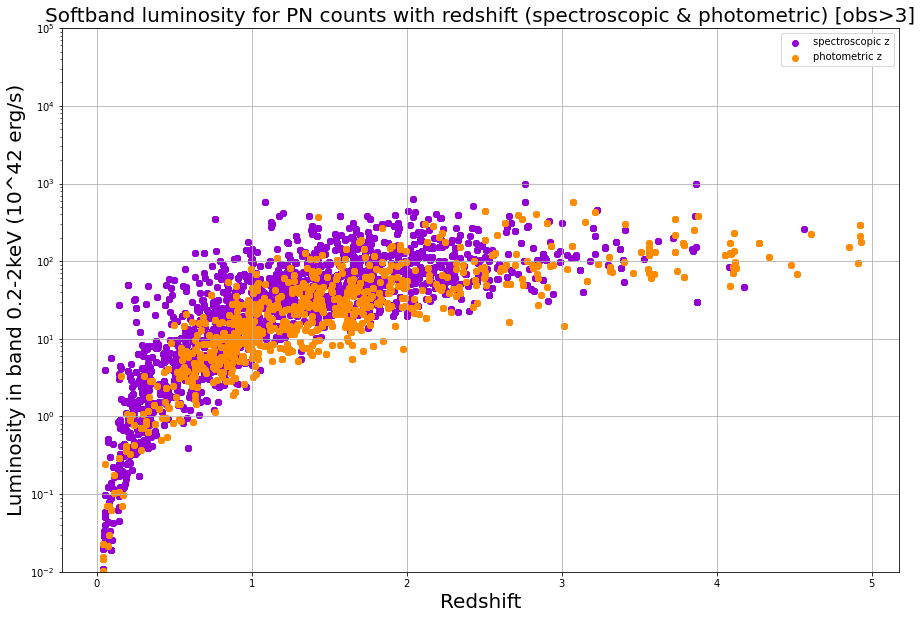
\includegraphics[width=0.8 \linewidth]{Figures/Lumi_Red.png}
 \caption{Λαμπρότητα ($ 10^{42}$ \textlatin{erg s}$^{-1}$) στις μαλακές ακτίνες Χ ($0.2-2$ \textlatin{keV}) συναρτήσει του \textlatin{redshift.}}
 \label{fig:LumiRed}
 \end{center}
 \end{figure*}
 
 
\begin{figure*}%
    \centering
    \subfloat{{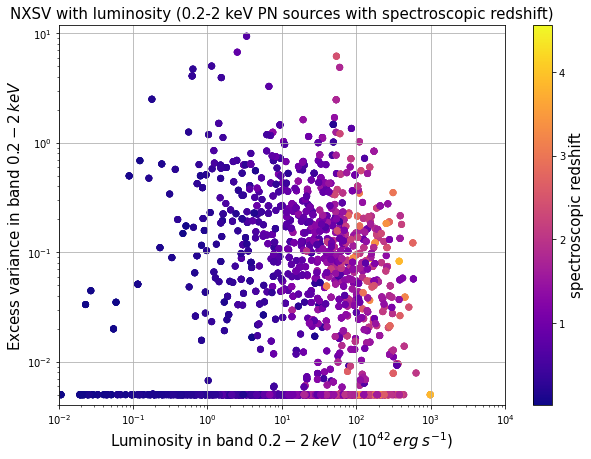
\includegraphics[width=0.9\linewidth]{Figures/NXSV_Lumi_zweight_SPECTRO.png} }}%
    \qquad
    \subfloat{{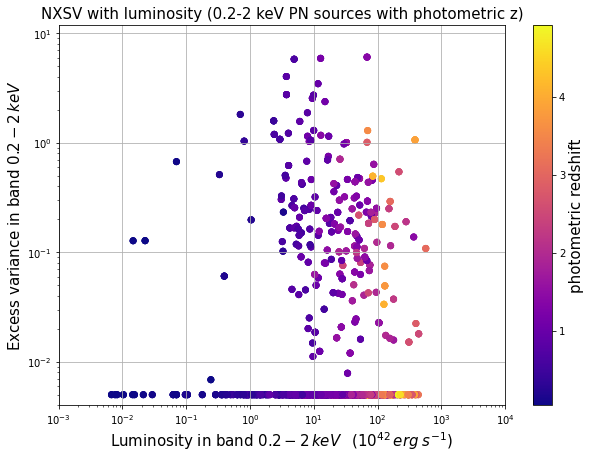
\includegraphics[width=0.9\linewidth]{Figures/NXSV_Lumi_zweight_PHOTO.png} }}%
    \caption{ \textlatin{NXSV} με λαμπρότητα κατά \textlatin{redshift.} Στο πάνω πάνελ οι πηγές για τις οποίες έχουμε φασματοσκοπική μέτρηση ερυθρομετατόπισης, ενώ στο κάτω πηγές για τις οποίες έχουμε μόνο φωτομετρική μέτρηση ερυθρομετατόπισης. Οι πηγές με \textlatin{NXSV}$<0.005$ απεικονίζονται στο επίπεδο 0.005.} \label{fig:NXSV-Zcbar}
\end{figure*}
%%%-----------------------------------------------------------%%%%
%%%-----------------------------------------------------------%%%%
%%%-----------------------------------------------------------%%%%

\section{Περιορισμός δείγματος και ανάλυση δεδομένων}

%{\color{red}: better to give values in years. Also wht you split them into near-equal time invtervals: Σκοπος είναι να μελετησουμε τη μεταβλοτητα των ΕΝΠ σε να χρονικο διαστημα 20 χρονων. Για το σκοπο αυτο διαλεγουμε πηγες που εχουν καμπλυλες φωτος με ομιομορφο sampling κατα τη διαρκεια των 19 χρονων κατα το οποιο το ΧΜΜ-ΧΜΛ εχει παρατηρηθει. Για το σκοπο αυτο χωριζουμε το συνολικο αριθμο παρτηρησεων σε 3 ομαδες οι ιποιες διαχωριζονται μεταξυ τους απο περιπου 4-5 ετη. Οι περιοδοι αυτοί αντιστοιχούν χονδιρκα στις 3 κυριες περιοδους κατα τις οποίες το ΧΜΜ-ΧΧΛ παρτηρηθηκε απλο το ΧΜΜ ωσ αποτελεσμα 3 μεγαωλων προγραμματων: XMM-XXL (arxes 2000, Pierre et al. 2006.), XMM-XXL (~2010) kai XMM Serves (telos tis dekaeties 2010. Απαιτουμε οι πηγες για τις οποιες θα υπολογισουμε ... να εχουνε τουλαχιστον μια παρατησρηση και στις 3 παραπακνβ περιοδουςσ....}. 
Θεωρούμε ότι η εγγενής μεταβλητότητα, την οποία εκτιμάμε με την $\sigma_{rms}^2$, είναι μια στοχαστική διαδικασία - έχει δηλαδή χαρακτήρα <<κόκκινου θορύβου>> \textlatin{(red noise)}. Τότε η \textlatin{NXSV} εξαρτάται από την διάρκεια της καμπύλης φωτός στο σύστημα ηρεμίας της πηγής. Καμπύλες φωτός πολύ μικρές σε έκταση κυριαρχούνται από στατιστικό θόρυβο και έτσι δεν είναι πολύ χρήσιμες στην μελέτη μας\cite{2017MNRAS.471.4398P}.\\
Οι συνολικές παρατηρήσεις όλων των πηγών εκτείνονται σε 19 έτη ($\sim 600$ \textlatin{Ms}). Σκοπός μας είναι να μελετήσουμε καμπύλες φωτός που να εκτείνονται σε όλο αυτό το χρονικό διάστημα (δηλαδή η κλίμακα χρόνου της εκτίμησης μεταβλητότητας είναι $\sim 10-20$ έτη) και τα σημεία τους να είναι όσο το δυνατόν ομοιόμορφα κατανεμημένα στην χρονοσειρά. Όμως, στον πλήρη πληθυσμό του πεδίου \textlatin{XMM-XXL-North} δεν έχουμε καμία καμπύλη φωτός μεμονομένης πηγής με περισσότερα από 15 σημεία από τον ανιχνευτή ΡΝ.\\
Για να εκλέξουμε όσο το δυνατόν μεγαλύτερες καμπύλες φωτός ομοιόμορφης συλλογής, χωρίζουμε τις συνολικές παρατηρήσεις σε τρεις εποχές- τρία χρονικά διαστήματα των 6-7 περίπου ετών ($\sim 200 $\textlatin{ Ms}) έκαστο. Ξεχωρίζουμε, λοιπόν, αφού έχουμε μετατρέψει τις χρονικές στιγμές έναρξης και λήξης κάθε παρατήρησης σε Ιουλιανή Εποχή (\textlatin{Julian Epoch}), τις εξής εποχές: 
\begin{itemize}
    \item Εποχή 1: [2000.0,2006.0] εκτείνεται σε 6 έτη, $\sim 189$ \textlatin{Ms}
    \item Εποχή 2: (2006.0,2014.0] εκτείνεται σε 8 έτη, $\sim 252$ \textlatin{Ms}
    \item Εποχή 3: (2014.0,2020.0] εκτείνεται σε 7 έτη, $\sim 221$ \textlatin{Ms}
\end{itemize}

Οι περίοδοι αυτές αντιστοιχούν σε αδρές γραμμές στις 3 κύριες περιόδους κατά τις οποίες το πεδίο \textlatin{XMM-XXL-North} παρατηρήθηκε από το τηλεσκόπιο \textlatin{XMM-Newton} ως αποτέλεσμα 3 μεγάλων προγραμμάτων: \textlatin{XMM-LSS} (αρχές 2000, \cite{2006MNRAS.372..591P}), \textlatin{XMM-XXL} ($\sim$2010, \cite{2016A&A...592A...1P}) kai \textlatin{XMM-SERVS} (προς το τέλος της δεκαετείας 2010, \cite{2018MNRAS.478.2132C}).

\begin{figure*} 
 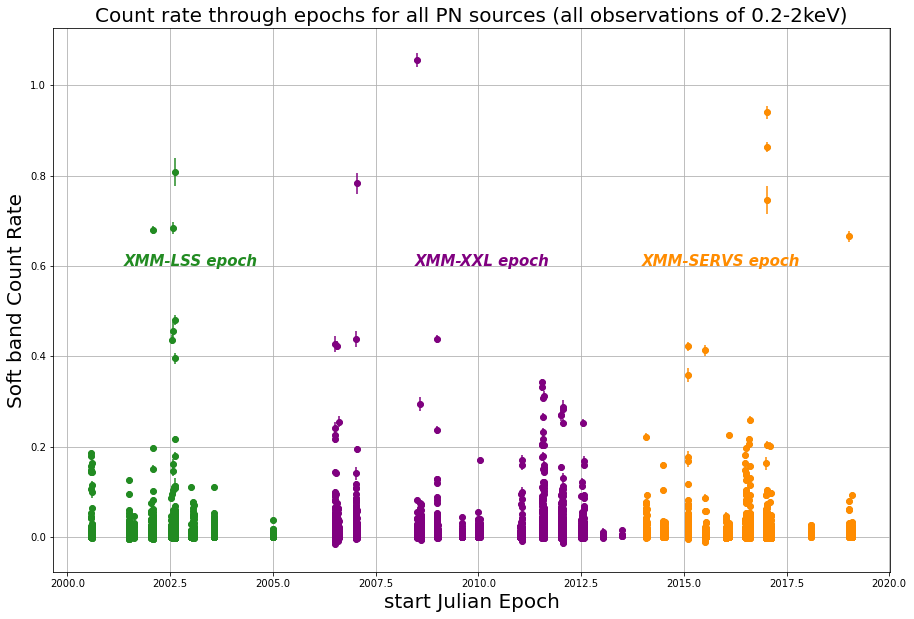
\includegraphics[width=0.9\linewidth]{Figures/Epochs.png}
 \caption{Οι συνολικές παρατηρήσεις εμπίπτουν σε τρία χρονικά διαστήματα- εποχές. Εδώ ο ρυθμός καταμέτρησης (\textlatin{CR}) με την χρονική τοποθέτηση της έναρξης κάθε παρατήρησης του ανιχνευτή \textlatin{PN} στην ερνεργειακή μπάντα $0.2-2$ \textlatin{keV}. }
 \label{fig:Epochs}
 \end{figure*}
 
Περιορίζουμε το δείγμα μας σε πηγές που έχουν παρατηρήσεις από τον ανιχνευτή \textlatin{PN} σε τρείς διαδοχικές διαφορετικές εποχές (όπως φαίνονται στο σχήμα \ref{fig:Epochs}), δηλαδή επιλέγουμε τις πηγές που έχουν μία τουλάχιστον παρατήρηση σε κάθε ένα από τα χρονικά διαστήματα που ορίσαμε, ετσι ώστε το δείγμα μας να έχει συνεχείς χρονικά παρατηρήσεις για μεγάλο χρονικό διάστημα. Η καμπύλη φωτός με το μεγαλύτερο παρατηρούμενο μήκος καλύπτει περίπου $17$ έτη, ενώ το μέσο μήκος καμπύλης φωτός καλύπτει $11$ έτη- αυτές είναι και οι χρονικές κλίμακες ($\sim 400$ \textlatin{Ms}) στις οποίες μελετάμε την μεταβλητότητα. 

Έχοντας επιλέξει πηγές με παρατηρήσεις σε τρείς διαδοχικές εποχές στην ενεργειακή μπάντα $0.2-2$ \textlatin{keV} από τον ανιχνευτή \textlatin{PN}, προκειμένου να αποκλείσουμε πηγές που έχουν πολύ θόρυβο (δηλαδή μικρό λόγο \textlatin{S/N}) επιλέγουμε να κάνουμε τα γραφήματα της  \textlatin{NXSV} με λαμπρότητα για πηγές με \textlatin{S/N}$>2$, \textlatin{S/N}$>3$, \textlatin{S/N}$>4$ (επιλέγοντας να βάλουμε ένα κάτω φραγμό στο \textlatin{S/N} του δείγματός μας, όπως φαίνεται στο σχήμα \ref{fig:NXSV_counts}).

 \begin{figure*}  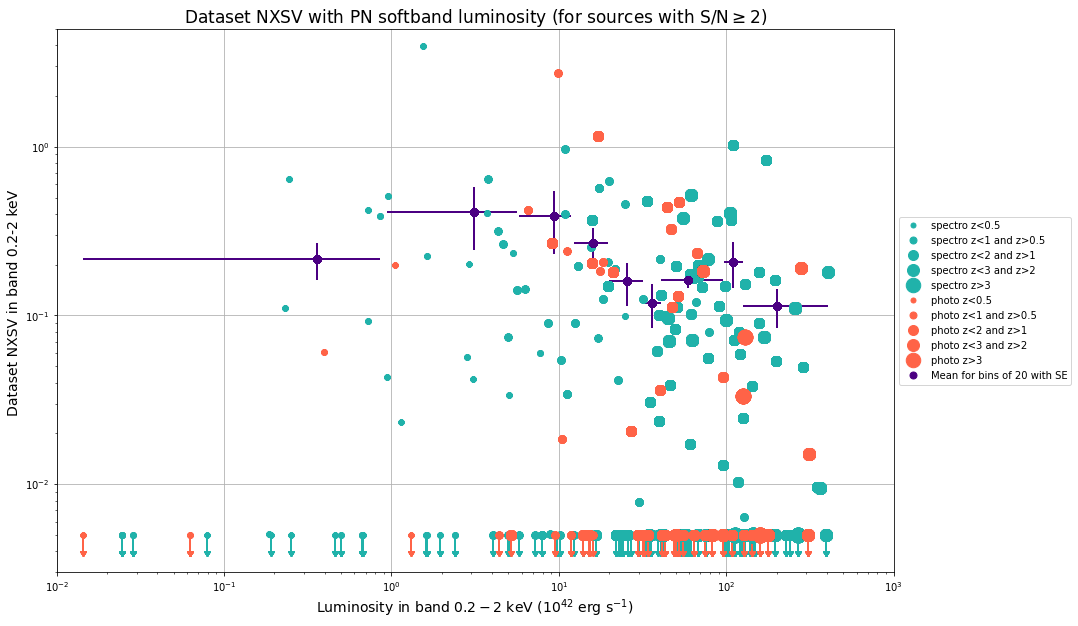
\includegraphics[width=1.12\linewidth]{Figures/NXSVclassic_sn2.png} \caption{ Η \textlatin{NXSV} με λαμπρότητα και \textlatin{binning} κατά λαμπρότητα σε \textlatin{bin} των 20 τουλάχιστον πηγών με διαφοροποίηση για \textlatin{redshift} και επιλέγοντας πηγές με \textlatin{S/N}$>2$. Η λαμπρότητα είναι προσαρμοσμένη στο σύστημα ηρεμίας της πηγής και σημειώνεται στον οριζόντιο λογαριθμικό άξονα σε κλίμακα $10^{42}$ \textlatin{erg s}$^{-1}$ για την παρατηρούμενη ενεργειακή μπάντα $0.2-2$ \textlatin{keV}. Η \textlatin{NXSV} είναι αδιάστατο μέγεθος και σημειώνεται στον κατακόρυφο λογαριθμικό άξονα για την παρατηρούμενη ενεργειακή μπάντα $0.2-2$ \textlatin{keV}.} \label{fig:NXSV_classic_sn2}
    \end{figure*}

 \begin{figure*}  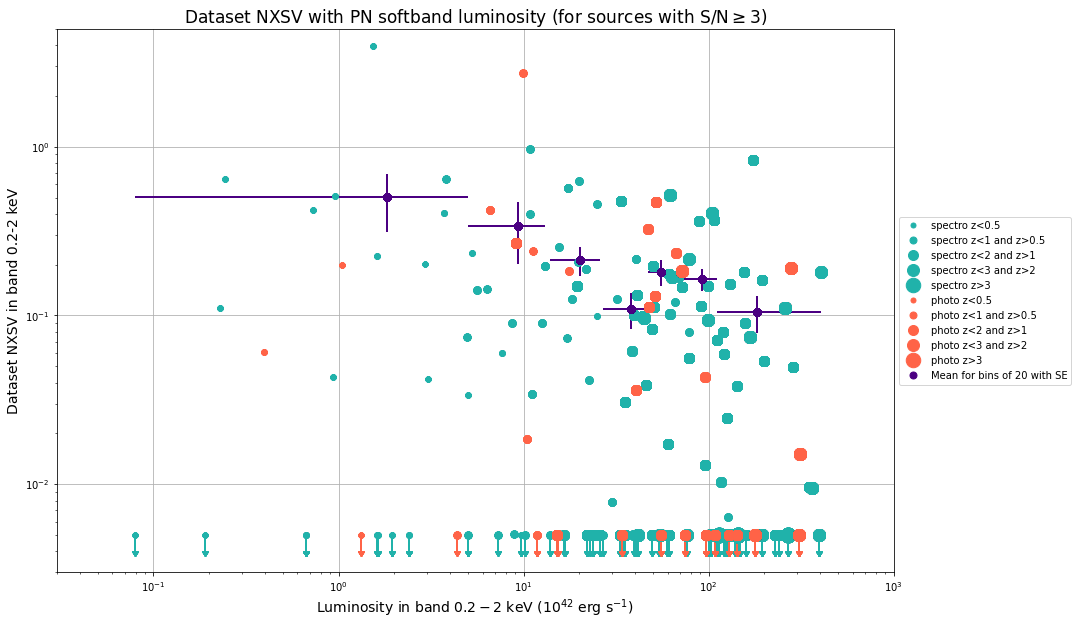
\includegraphics[width=1.12\linewidth]{Figures/NXSVclassic_sn3.png} \caption{ Η \textlatin{NXSV} με λαμπρότητα και \textlatin{binning} κατά λαμπρότητα σε \textlatin{bin} των 20 τουλάχιστον πηγών με διαφοροποίηση για \textlatin{redshift} και επιλέγοντας πηγές με \textlatin{S/N}$>3$. Η λαμπρότητα είναι προσαρμοσμένη στο σύστημα ηρεμίας της πηγής και σημειώνεται στον οριζόντιο λογαριθμικό άξονα σε κλίμακα $10^{42}$ \textlatin{erg s}$^{-1}$ για την παρατηρούμενη ενεργειακή μπάντα $0.2-2$ \textlatin{keV}. Η \textlatin{NXSV} είναι αδιάστατο μέγεθος και σημειώνεται στον κατακόρυφο λογαριθμικό άξονα για την παρατηρούμενη ενεργειακή μπάντα $0.2-2$ \textlatin{keV}.}  \label{fig:NXSV_classic_sn3}
   \end{figure*}

 \begin{figure*}  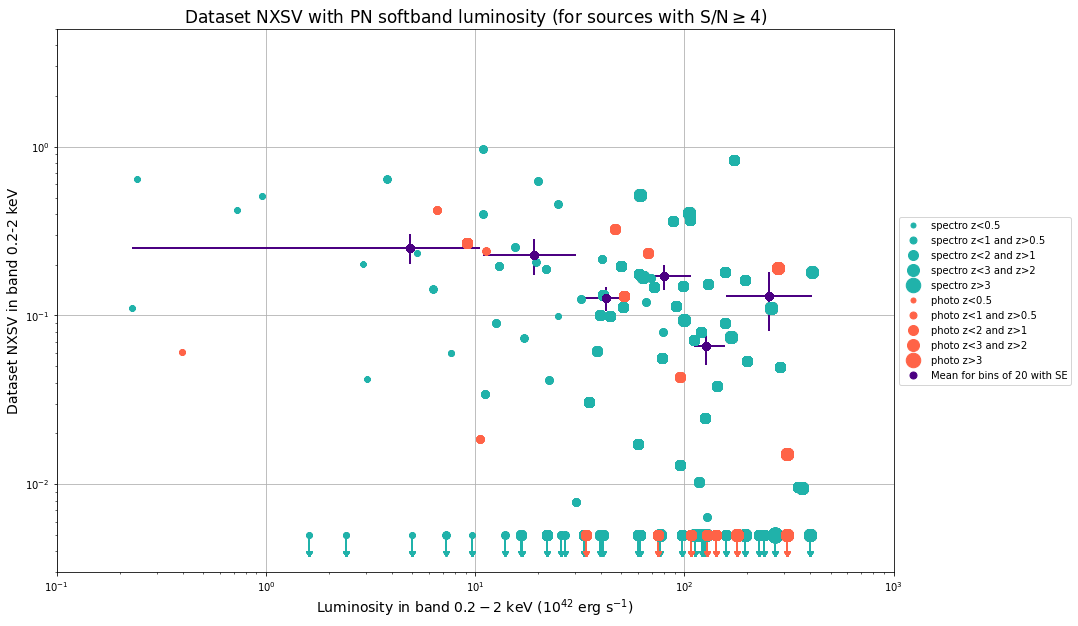
\includegraphics[width=1.12\linewidth]{Figures/NXSVclassic_sn4.png} \caption{ Η \textlatin{NXSV} με λαμπρότητα και \textlatin{binning} κατά λαμπρότητα σε \textlatin{bin} των 20 τουλάχιστον πηγών με διαφοροποίηση για \textlatin{redshift} και επιλέγοντας πηγές με \textlatin{S/N}$>4$. Η λαμπρότητα είναι προσαρμοσμένη στο σύστημα ηρεμίας της πηγής και σημειώνεται στον οριζόντιο λογαριθμικό άξονα σε κλίμακα $10^{42}$ \textlatin{erg  s}$^{-1}$ για την παρατηρούμενη ενεργειακή μπάντα $0.2-2$ \textlatin{keV}. Η \textlatin{NXSV} είναι αδιάστατο μέγεθος και σημειώνεται στον κατακόρυφο λογαριθμικό άξονα για την παρατηρούμενη ενεργειακή μπάντα $0.2-2$ \textlatin{keV}.} \label{fig:NXSV_classic_sn4}
  \end{figure*}
 
Στα σχήματα (\ref{fig:NXSV_classic_sn2}, \ref{fig:NXSV_classic_sn3}, \ref{fig:NXSV_classic_sn4}) βλέπουμε την κατανομή της \textlatin{NXSV} όπως την υπολογίσαμε για κάθε πηγή σύμφωνα με τον τύπο (\ref{eq:NXSV}) με την λαμπρότητα στο αδρανειακό σύστημα ηρεμίας που καταγράφουμε  στις μαλακές ακτίνες Χ ($0.2-2$ \textlatin{keV}) σύμφωνα με τις σχέσεις (\ref{eq:LumiFluxRest},\ref{eq:DL}, \ref{eq:Dcmr})- η οποία υπολογίστηκε από φασματοσκοπικές μετρήσεις \textlatin{redshift} για κάθε πηγή, ή φωτομετρικό για τις πηγές που δεν διέθεταν φασματοσκοπικό. Οι πηγές για τις οποίες υπολογίσαμε τιμή τιμή \textlatin{NXSV} μικρότερη από $0.005$ εμφανίζονται στο επίπεδο $0.005$ του γραφήματος για λόγους εξοικονόμησης χώρου. \\
Επίσης, έχουμε ομαδοποιήσει (\textlatin{binning}) τις πηγές αρχίζοντας από τις χαμηλότερες λαμπρότητες και φτιάχνοντας ομάδες (\textlatin{bin}) των 20 πηγών με σκοπό να αναπαραστήσουμε την μέση τιμή του κάθε \textlatin{bin} ώστε να φανεί η συσχέτιση της \textlatin{ensemble NXSV} με την λαμπρότητα πιο καθαρά (έχει επισημαθεί ότι η \textlatin{ensemble NXSV} δείνει χρήσιμα αποτελέσματα για συλλογή τουλάχιστον 20 καμπύλων φωτός \cite{2013ApJ...771....9A}). Ορισμένες ομάδες (οι δύο ομάδες με τις υψηλότερες λαμπρότητες για \textlatin{S/N}$>2$, και η μια ομάδα με την υψηλότερη λαμπρότητα για \textlatin{S/N}$>3$) περιέχουν περισσότερες από 20 πηγές. Στον υπολογισμό της μέσης τιμής \textlatin{NXSV}, δηλαδή της \textlatin{ensemble NXSV} για κάθε ομάδα, έχουμε υπολογίσει τον καθαρό αριθμητικό μέσο της \textlatin{NXSV} κάθε πηγής. Στον υπολογισμό αυτόν δεν αποκλείσαμε πηγές με μηδενική ή αρνητική τιμή $\sigma_{rms}^2$, διότι τότε θα εισαγάγαμε  μεροληψία \textlatin{(bias)} στο δείγμα\cite{2017MNRAS.471.4398P}\cite{2013ApJ...771....9A}. Η μέση τιμή αυτή είναι η \textlatin{ensemble NXSV} για κάθε ομάδα πηγών και εκτιμά καλώς\cite{2017MNRAS.471.4398P}\cite{2013ApJ...771....9A} την εγγενή μεταβλητότητα όλων των πηγών (δεδομένου ότι όλες οι πηγές σε κάθε \textlatin{bin} λαμπρότητας έχουν παρόμοιες ιδιότητες και χαρακτηριστικά). \\
Οι σημάνσεις σφαλμάτων έγιναν ως εξής: το σφάλμα στις λαμπρότητες εκτείνεται από την χαμηλοτερη εως υψηλότερη τιμή λαμπρότητας των πηγών που περιέχονται στο \textlatin{bin} (είναι δηλαδή το πλάτος του \textlatin{bin}), το σφάλμα στην \textlatin{NXSV} του κάθε \textlatin{bin} είναι σφάλμα μέσης τιμής \textlatin{(standard errror)}. Για κάθε \textlatin{bin} των 20 (ή παραπάνω) πηγών:
$$ \overline{\sigma_{rms}}_{,err}  =\dfrac{ \sqrt{ \sum_{j=1}^{20}(\sigma_{rms, j}- \overline{\sigma_{rms}})^2}}{(20-1)(20)}$$

Εξετάζοντας τα σχήματα (\ref{fig:NXSV_classic_sn2}, \ref{fig:NXSV_classic_sn3}, \ref{fig:NXSV_classic_sn4}), παρατηρούμε αντισυσχέτιση (\textlatin{anticorrelation}) των μεγεθών αυτών, το οποίο είναι συνεπές με αντίστοιχες έρευνες \textlatin{AGN} που έχουν παρουσιαστεί σε εργασίες πάνω σε διαφορετικά πεδία (π.χ. \textlatin{CDF-S}) και διαφορετικές χρονικές κλίμακες \cite{2017MNRAS.471.4398P}. 

Προκειμένου να ελατώσουμε τον θόρυβο στο δείγμα, αλλά και να έχουμε αρκετές πηγές ώστε να δουλέψουμε, επιλέγουμε από εδώ κι έπειτα να χρησιμοποιήσουμε τον περιορισμό \textlatin{S/N}$>3$ για τον λόγο σήματος προς θόρυβο του δείγματός μας, αυτό περιορίζει δραστικά το δείγμα μας σε 175 πηγές.

Έτσι για \textlatin{S/N}$>3$, με αρχική υπόθεση ($P_{null}$) ότι δεν υπάρχει συσχέτιση μεταξύ της κλασσικά υπολογισμένης \textlatin{NXSV} $\sigma_{rms}^2$ και του λογαρίθμου της λαμπρότητας σε μαλακές ακτίνες Χ $\log L_X$, για το στατιστικό τεστ \textlatin{Kendall's} $\tau$ ο συντελεστής συσχέτισης $\sigma_{rms}^2$ και $\log L_X$ για τις πηγές με φασματοσκοπικό $z$ είναι $\tau_{spectro} =-0.092$ ενώ για τις πηγές με φωτομετρικό $z$ είναι $\tau_{photo} = -0.141$ τα οποία αντιστοιχούν σε $P_{null, spectro} = 0.101$ kai $P_{null, photo} = 0.266$. Τα αρνητικά πρόσημα στους συντελεστές υποδηλώνουν φθίνουσα μονότονη σχέση, ενώ θεωρούμε ότι υπάρχει (αντι)συσχέτιση αν έχουμε τιμή σημαντικότητας $P_{null}<5\%$, το οποίο δεν ισχύει ούτε για τις πηγές με φασματοσκοπικό ούτε και για τις πηγές με φωτομετρικό $z$.
Σε πλήρη αναλογία, το στατιστικό τεστ \textlatin{Spearman's rank} δίνει συντελεστή συσχέτισης $\rho_{spectro} =-0.134$ me $P_{null, spectro} = 0.110>0.05$ για τις πηγές με φασματοσκοπικό \textlatin{redshift} kai $\rho_{photo} = -0.211$ me $P_{null, photo} =0.246>0.05$ για τις πηγές με φωτομετρικό \textlatin{redshift}- δηλαδή επιβεβαιώνεται η μη συσχέτιση της $\sigma_{rms}^2$ των πηγών με την λογαριθμική λαμπρότητα $\log L_X$. \\
Για το σύνολο των πηγών (ανεξαρτήτως διαχωρισμού \textlatin{redshift}), το τεστ \textlatin{Kendall's} $\tau$ δίνει συντελεστή συσχέτισης $\tau_{tot} = -0.098$ me $P_{null, tot}= 0.053 $ (οριακά $>0.05$) ενώ το τεστ \textlatin{Spearman's rank} δίνει συντελεστή συσχέτισης $\rho_{tot} = -0.145$ me $P_{null, tot} = 0.055$ (οριακά $>0.05$), οπότε και στο σύνολο των πηγών δεν επιβεβαιώνεται η αντισυσχέτιση σε επίπεδο σημαντικότητας $95\%$\footnote{Η διεξαγωγή των στατιστικών ελέγχων έγινε με τις μεθόδους \textlatin{scipy.stats.kendalltau} kai \textlatin{scipy.stats.spearmanr} της βιβλιοθήκης \textlatin{SciPy.}}, (όμως επιβεβαιώνεται σε επίπεδο σημαντικότητας $90\%$). \\
Για την \textlatin{ensemble NXSV} ο έλεγχος \textlatin{Kendall's} $\tau$ δίνει συντελεστή συσχέτισης $\tau = -0.810$ και ο έλεγχος \textlatin{Spearman's rank} δίνει συντελεστή συσχέτισης $\rho= -0.893$ me τιμές σημαντικότητας $P_{null, \tau} =0.011<0.05$ kai $P_{null, \rho} = 0.007<0.05$ αντίστοιχα. Έχουμε δηλαδή ισχυρή ένδειξη αντισυσχέτισης της \textlatin{ensemble NXSV} με την λογαριθμική λαμπρότητα.\\ 
Προσαρμόζουμε γραμμική σχέση μέσω γραμμικής παλινδρόμησης (\textlatin{linear regression}) sta δεδομένα και βρίσκουμε κλίση $-0.11$ (δηλαδή $\sigma_{rms}^2\propto L_X^{-0.11}$) με σφάλμα μέσης τιμής $StErr = 0.04 $ για τις όλες τις πηγές μαζί. Επαναλαμβάνουμε για την \textlatin{ensemble NXSV} και βρίσκουμε και πάλι κλίση $-0.11$ (δηλαδή $\sigma_{rms, ensemble}^2= \overline{\sigma_{rms}^2}\propto L_X^{-0.11}$) με σφάλμα μέσης τιμής $StErr = 0.01 $, έτσι επιβεβαιώνεται η αντισυσχέτιση \footnote{Η γραμμική παλινδρόμηση έγινε με την μέθοδο \textlatin{scipy.stats.linregress} της βιβλιοθήκης \textlatin{SciPy.}}.

Το συμπέρασμα της αντισυσχέτισης του πλάτους μεταβλητότητας $\sigma_{rms, ensemble}^2$ με την λογαριθμική λαμπρότητα $\log L_X$ στις ενέργειες $0.2-2$ \textlatin{keV}, στο οποίο καταλήγουμε λαμβάνοντας υπ> όψιν τις τιμές μόνο (χωρίς να συνυπολογίζουμε σφάλματα) μας υποδεικνύει πως οι \textlatin{AGN} με μεγαλύτερη λαμπρότητα είναι λιγότερο μεταβλητοί.\\
Αντισυσχέτιση πλάτους μεταβλητότητας \textlatin{AGN} με λαμπρότητα σημαίνει πώς οι λαμπρότεροι \textlatin{AGN} είναι λιγότερο μεταβλητοί, το οποίο από την σχέση \textlatin{Eddington} συνεπάγεται πως οι \textlatin{AGN} με την μεγαλύτερη μάζα μελανής οπής είναι οι λιγότερο μεταβλητοί. Αν δεχτούμε ότι η κύρια αιτία μεταβλητότητας είναι αστάθειες στον δίσκο προσάυξησης, τότε η αντισυσχέτιση θα υποδείκνυε ότι οι \textlatin{AGN} με τις μεγαλύτερες μάζες μελανής οπής είναι αυτοί με τις λιγότερες αστάθειες στην διαδικασία προσαύξησης.\\
Παρ> όλα αυτά, η μεγάλη αβεβαιότητα μας εμποδίζει να βγάλουμε οριστικό συμπέρασμα για την (αντι)συσχέτιση ή μη του πλάτους μεταβλητότητας με την λαμπρότητα στο ενεργειακό παράθυρο $0.2-2$ \textlatin{keV}. 


%{\color{red} AGE: (Ερμηνεια αντισυσχέτισης συντομα εδω και στη συνεχεια στη συζητηση!!!!!). }
